\documentclass[tikz,border=10pt]{standalone}
\usepackage{tikz}
\usepackage{amsmath}
\usetikzlibrary{shapes.geometric,positioning,arrows.meta,decorations.pathreplacing}

\begin{document}
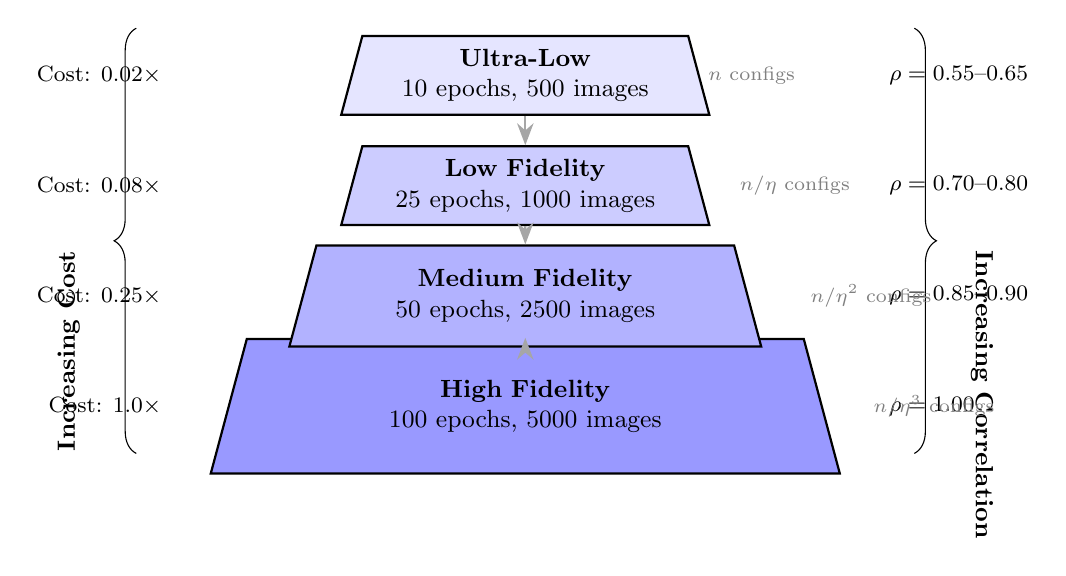
\begin{tikzpicture}[
    level/.style={trapezium, trapezium angle=75, draw, thick, minimum height=1cm,
                  text width=3.5cm, align=center, font=\small},
    arrow/.style={-{Stealth[scale=1.2]}, thick},
    brace/.style={decorate, decoration={brace, amplitude=8pt, raise=4pt}}
]

% Fidelity levels (pyramid from bottom to top)
\node[level, fill=blue!40, minimum width=8cm] (high) at (0,0)
    {\textbf{High Fidelity}\\100 epochs, 5000 images};

\node[level, fill=blue!30, minimum width=6cm] (med) at (0,1.4)
    {\textbf{Medium Fidelity}\\50 epochs, 2500 images};

\node[level, fill=blue!20, minimum width=4.5cm] (low) at (0,2.8)
    {\textbf{Low Fidelity}\\25 epochs, 1000 images};

\node[level, fill=blue!10, minimum width=3cm] (ultra) at (0,4.2)
    {\textbf{Ultra-Low}\\10 epochs, 500 images};

% Left side: Cost annotations
\node[anchor=east, font=\footnotesize] at (-4.5,0) {Cost: $1.0\times$};
\node[anchor=east, font=\footnotesize] at (-4.5,1.4) {Cost: $0.25\times$};
\node[anchor=east, font=\footnotesize] at (-4.5,2.8) {Cost: $0.08\times$};
\node[anchor=east, font=\footnotesize] at (-4.5,4.2) {Cost: $0.02\times$};

% Right side: Correlation annotations
\node[anchor=west, font=\footnotesize] at (4.5,0) {$\rho = 1.00$};
\node[anchor=west, font=\footnotesize] at (4.5,1.4) {$\rho = 0.85\text{--}0.90$};
\node[anchor=west, font=\footnotesize] at (4.5,2.8) {$\rho = 0.70\text{--}0.80$};
\node[anchor=west, font=\footnotesize] at (4.5,4.2) {$\rho = 0.55\text{--}0.65$};

% Left brace and label
\draw[brace] (-4.8,-0.6) -- (-4.8,4.8);
\node[anchor=east, rotate=90, font=\small\bfseries] at (-5.8,2.1) {Increasing Cost};

% Right brace and label
\draw[brace, decoration={mirror}] (4.8,-0.6) -- (4.8,4.8);
\node[anchor=west, rotate=-90, font=\small\bfseries] at (5.8,2.1) {Increasing Correlation};

% Arrows showing information flow
\draw[arrow, color=gray!70] (ultra.south) -- (low.north);
\draw[arrow, color=gray!70] (low.south) -- (med.north);
\draw[arrow, color=gray!70] (med.south) -- (high.north);

% Number of configurations annotations
\node[anchor=west, font=\scriptsize, color=gray] at (2.2,4.2) {$n$ configs};
\node[anchor=west, font=\scriptsize, color=gray] at (2.6,2.8) {$n/\eta$ configs};
\node[anchor=west, font=\scriptsize, color=gray] at (3.5,1.4) {$n/\eta^2$ configs};
\node[anchor=west, font=\scriptsize, color=gray] at (4.3,0) {$n/\eta^3$ configs};

\end{tikzpicture}
\end{document}
